\begin{frame}
    \only<1,2,3>{\frametitle{Trade-off in Tree Search}}
    \only<4>{\frametitle{Trade-off in Tree Search - Meet in the Middle}}
    \only<1>{
    \begin{itemize}
        \item Bob can send all $u^d$ prefixes to Alice ($u$ being each dimension's bit length).
        \item In each step, Alice discovers one new bit by searching $2$ children.
    \end{itemize}
    }
    \only<2>{
    \begin{itemize}
        \item If Bob does not send the near-last prefix of the last dimension: $u^{d-1} \cdot (u-1)$ prefixes.
        \item In the last step, Alice searches $4$ children to discover the final bits.
    \end{itemize}
    }
    \only<3>{
    \begin{itemize}
        \item If Bob skips $2$ intermediate prefixes: $u^{d-1} \cdot (u-2)$ prefixes sent.
        \item In the last step, Alice searches $8$ children to discover the final bits.
    \end{itemize}
    }
    \only<4>{
    \begin{itemize}
        \item Bob can choose the first $k$ dimensions to send all prefixes: $u^k$ prefixes sent.
        \item Alice needs $2^{u(d-k)}$ searches to discover the remaining bits.
    \end{itemize}
    }

    \centering
    \only<1>{
    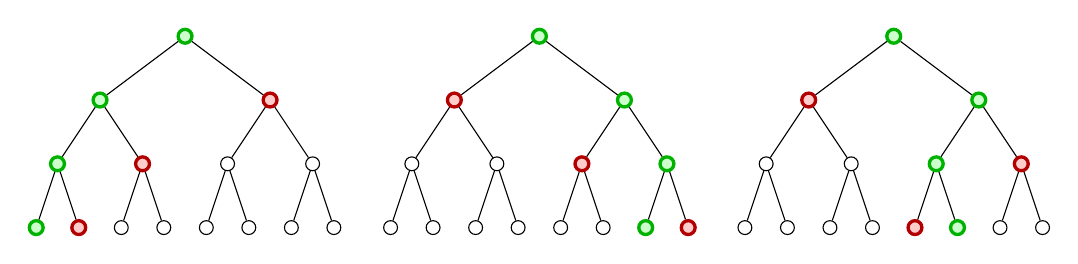
\begin{tikzpicture}[grow=down,level distance=0.9cm,
        base/.style={circle,draw,minimum size=5pt,inner sep=1.2pt},
        marked/.style={base,draw=green!70!black,fill=green!20,very thick},
        failed/.style={base,draw=red!70!black,fill=red!20,very thick},
        every node/.style=base,
        level 1/.style={sibling distance=2.4cm},
        level 2/.style={sibling distance=1.2cm},
        level 3/.style={sibling distance=0.6cm}]
        % Left tree
        \begin{scope}[xshift=-4.5cm,scale=0.9]
            \node[marked] (r) {}
                child { node[marked] (l1) {}
                    child { node[marked] (l2a) {} child { node[marked] (l3a) {} } child { node[failed] {} } }
                    child { node[failed] (l2b) {} child { node {} } child { node {} } }
                }
                child { node[failed] (r1) {}
                    child { node (r2a) {} child { node {} } child { node {} } }
                    child { node (r2b) {} child { node {} } child { node {} } }
                };
        \end{scope}
        % Middle tree
        \begin{scope}[xshift=0cm,scale=0.9]
            \node[marked] (r) {}
                child { node[failed] (l1) {}
                    child { node (l2a) {} child { node {} } child { node {} } }
                    child { node (l2b) {} child { node {} } child { node {} } }
                }
                child { node[marked] (r1) {}
                    child { node[failed] (r2a) {} child { node {} } child { node {} } }
                    child { node[marked] (r2b) {} child { node[marked] (r3d) {} } child { node[failed] {} } }
                };
        \end{scope}
        % Right tree
        \begin{scope}[xshift=4.5cm,scale=0.9]
            \node[marked] (r) {}
                child { node[failed] (l1) {}
                    child { node (l2a) {} child { node {} } child { node {} } }
                    child { node (l2b) {} child { node {} } child { node {} } }
                }
                child { node[marked] (r1) {}
                    child { node[marked] (r2a) {} child { node[failed] {} } child { node[marked] (r3b) {} } }
                    child { node[failed] (r2b) {} child { node {} } child { node {} } }
                };
        \end{scope}
    \end{tikzpicture}
    }

    \only<2>{
    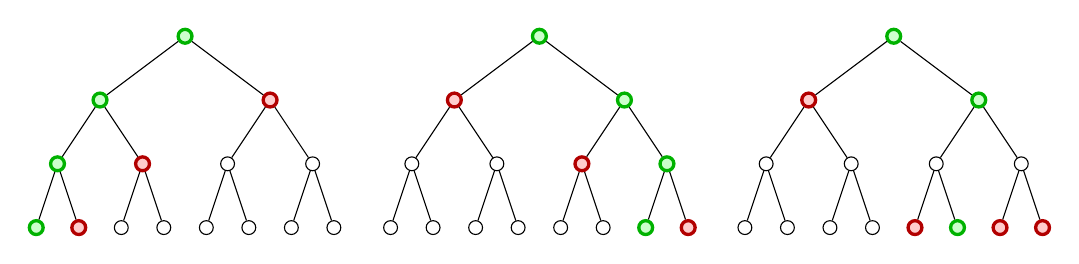
\begin{tikzpicture}[grow=down,level distance=0.9cm,
        base/.style={circle,draw,minimum size=5pt,inner sep=1.2pt},
        marked/.style={base,draw=green!70!black,fill=green!20,very thick},
        failed/.style={base,draw=red!70!black,fill=red!20,very thick},
        every node/.style=base,
        level 1/.style={sibling distance=2.4cm},
        level 2/.style={sibling distance=1.2cm},
        level 3/.style={sibling distance=0.6cm}]
        % Left tree
        \begin{scope}[xshift=-4.5cm,scale=0.9]
            \node[marked] (r) {}
                child { node[marked] (l1) {}
                    child { node[marked] (l2a) {} child { node[marked] (l3a) {} } child { node[failed] {} } }
                    child { node[failed] (l2b) {} child { node {} } child { node {} } }
                }
                child { node[failed] (r1) {}
                    child { node (r2a) {} child { node {} } child { node {} } }
                    child { node (r2b) {} child { node {} } child { node {} } }
                };
        \end{scope}
        % Middle tree
        \begin{scope}[xshift=0cm,scale=0.9]
            \node[marked] (r) {}
                child { node[failed] (l1) {}
                    child { node (l2a) {} child { node {} } child { node {} } }
                    child { node (l2b) {} child { node {} } child { node {} } }
                }
                child { node[marked] (r1) {}
                    child { node[failed] (r2a) {} child { node {} } child { node {} } }
                    child { node[marked] (r2b) {} child { node[marked] (r3d) {} } child { node[failed] {} } }
                };
        \end{scope}
        % Right tree
        \begin{scope}[xshift=4.5cm,scale=0.9]
            \node[marked] (r) {}
                child { node[failed] (l1) {}
                    child { node (l2a) {} child { node {} } child { node {} } }
                    child { node (l2b) {} child { node {} } child { node {} } }
                }
                child { node[marked] (r1) {}
                    child { node (r2a) {} child { node[failed] {} } child { node[marked] (r3b) {} } }
                    child { node (r2b) {} child { node[failed] {} } child { node[failed] {} } }
                };
        \end{scope}
    \end{tikzpicture}
    }

    \only<3>{
    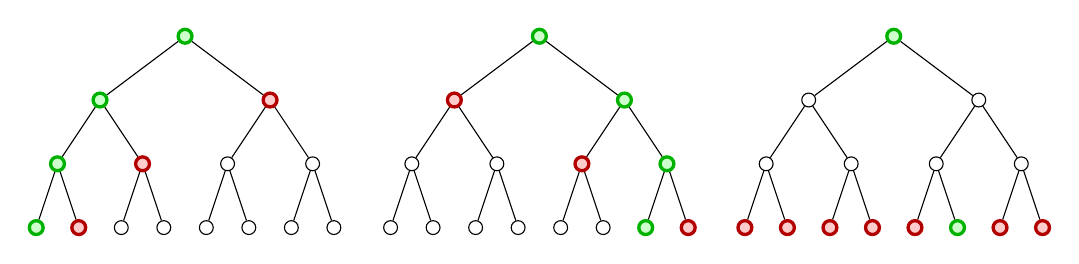
\begin{tikzpicture}[grow=down,level distance=0.9cm,
        base/.style={circle,draw,minimum size=5pt,inner sep=1.2pt},
        marked/.style={base,draw=green!70!black,fill=green!20,very thick},
        failed/.style={base,draw=red!70!black,fill=red!20,very thick},
        every node/.style=base,
        level 1/.style={sibling distance=2.4cm},
        level 2/.style={sibling distance=1.2cm},
        level 3/.style={sibling distance=0.6cm}]
        % Left tree
        \begin{scope}[xshift=-4.5cm,scale=0.9]
            \node[marked] (r) {}
                child { node[marked] (l1) {}
                    child { node[marked] (l2a) {} child { node[marked] (l3a) {} } child { node[failed] {} } }
                    child { node[failed] (l2b) {} child { node {} } child { node {} } }
                }
                child { node[failed] (r1) {}
                    child { node (r2a) {} child { node {} } child { node {} } }
                    child { node (r2b) {} child { node {} } child { node {} } }
                };
        \end{scope}
        % Middle tree
        \begin{scope}[xshift=0cm,scale=0.9]
            \node[marked] (r) {}
                child { node[failed] (l1) {}
                    child { node (l2a) {} child { node {} } child { node {} } }
                    child { node (l2b) {} child { node {} } child { node {} } }
                }
                child { node[marked] (r1) {}
                    child { node[failed] (r2a) {} child { node {} } child { node {} } }
                    child { node[marked] (r2b) {} child { node[marked] (r3d) {} } child { node[failed] {} } }
                };
        \end{scope}
        % Right tree
        \begin{scope}[xshift=4.5cm,scale=0.9]
            \node[marked] (r) {}
                child { node (l1) {}
                    child { node (l2a) {} child { node[failed] {} } child { node[failed] {} } }
                    child { node (l2b) {} child { node[failed] {} } child { node[failed] {} } }
                }
                child { node (r1) {}
                    child { node (r2a) {} child { node[failed] {} } child { node[marked] (r3b) {} } }
                    child { node (r2b) {} child { node[failed] {} } child { node[failed] {} } }
                };
        \end{scope}
    \end{tikzpicture}
    }

    \only<4>{
    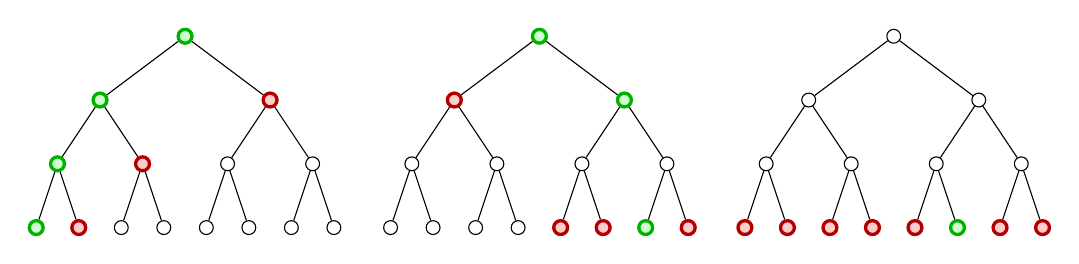
\begin{tikzpicture}[grow=down,level distance=0.9cm,
        base/.style={circle,draw,minimum size=5pt,inner sep=1.2pt},
        marked/.style={base,draw=green!70!black,fill=green!20,very thick},
        failed/.style={base,draw=red!70!black,fill=red!20,very thick},
        every node/.style=base,
        level 1/.style={sibling distance=2.4cm},
        level 2/.style={sibling distance=1.2cm},
        level 3/.style={sibling distance=0.6cm}]
        % Left tree
        \begin{scope}[xshift=-4.5cm,scale=0.9]
            \node[marked] (r) {}
                child { node[marked] (l1) {}
                    child { node[marked] (l2a) {} child { node[marked] (l3a) {} } child { node[failed] {} } }
                    child { node[failed] (l2b) {} child { node {} } child { node {} } }
                }
                child { node[failed] (r1) {}
                    child { node (r2a) {} child { node {} } child { node {} } }
                    child { node (r2b) {} child { node {} } child { node {} } }
                };
        \end{scope}
        % Middle tree
        \begin{scope}[xshift=0cm,scale=0.9]
            \node[marked] (r) {}
                child { node[failed] (l1) {}
                    child { node (l2a) {} child { node {} } child { node {} } }
                    child { node (l2b) {} child { node {} } child { node {} } }
                }
                child { node[marked] (r1) {}
                    child { node (r2a) {} child { node[failed] {} } child { node[failed] {} } }
                    child { node (r2b) {} child { node[marked] (r3d) {} } child { node[failed] {} } }
                };
        \end{scope}
        % Right tree
        \begin{scope}[xshift=4.5cm,scale=0.9]
            \node (r) {}
                child { node (l1) {}
                    child { node (l2a) {} child { node[failed] {} } child { node[failed] {} } }
                    child { node (l2b) {} child { node[failed] {} } child { node[failed] {} } }
                }
                child { node (r1) {}
                    child { node (r2a) {} child { node[failed] {} } child { node[marked] (r3b) {} } }
                    child { node (r2b) {} child { node[failed] {} } child { node[failed] {} } }
                };
        \end{scope}
    \end{tikzpicture}
    }
\end{frame}

\begin{frame}
    \only<1>{\frametitle{Trade-off in Tree Search - Meet in the Middle}}
    \only<2,3>{\frametitle{Trade-off in Tree Search - Better Pruning}}
    \begin{itemize}
        \only<1>{\item The previous slide is a bit misleading!}
        \only<2,3>{\item Bob can slice differently to help Alice with more efficient search.}
    \end{itemize}
    \centering
    \only<1>{
    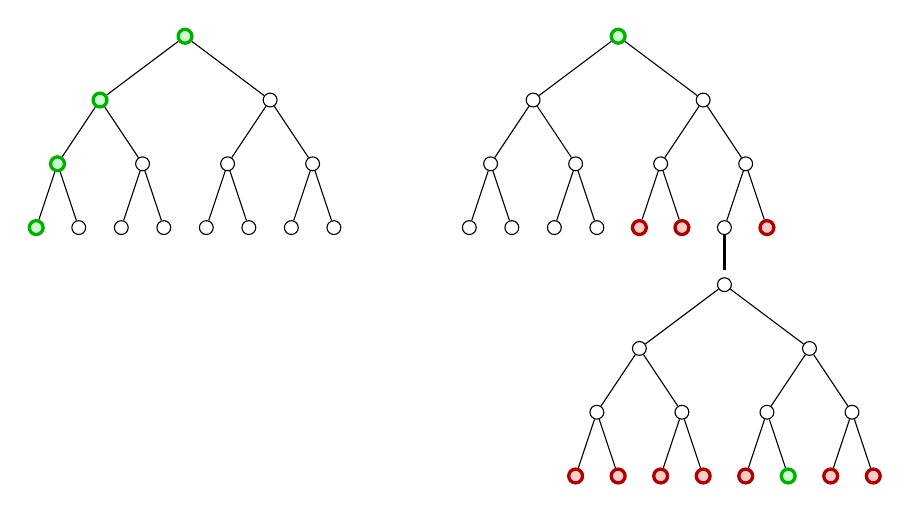
\begin{tikzpicture}[grow=down,level distance=0.9cm,
        base/.style={circle,draw,minimum size=5pt,inner sep=1.2pt},
        marked/.style={base,draw=green!70!black,fill=green!20,very thick},
        failed/.style={base,draw=red!70!black,fill=red!20,very thick},
        every node/.style=base,
        level 1/.style={sibling distance=2.4cm},
        level 2/.style={sibling distance=1.2cm},
        level 3/.style={sibling distance=0.6cm}]
        % First tree on the left
        \begin{scope}[xshift=-3cm,scale=0.9]
            \node[marked] (a0) {}
                child { node[marked] (a1) {}
                    child { node[marked] (a2) {} child { node[marked] (a3) {} } child { node {} } }
                    child { node {} child { node {} } child { node {} } }
                }
                child { node {} child { node {} child { node {} } child { node {} } } child { node {} child { node {} } child { node {} } } };
        \end{scope}

        % Second tree in the middle; its marked leaf becomes the root of the third tree
        \begin{scope}[xshift=2.5cm,scale=0.9]
            \node[marked] (b0) {}
                child { node {} 
                    child { node {} child { node {} } child { node {} } } 
                    child { node {} child { node {} } child { node {} } } }
                child { node (b1) {}
                    child { node {} child { node[failed] (b3) {} } child { node[failed] (b4) {} } }
                    child { node (b2) {}
                        child { node (b5) {}}
                        child { node[failed] (b6) {} }
                    }
                };

            % Third tree hanging from the marked leaf b3
            \begin{scope}[shift={(b5.south)},yshift=-0.7cm]
                \node (c0) {}
                    child { node (c1) {}
                        child { node (c2) {} child { node[failed] {} } child { node[failed] {} } }
                        child { node {} child { node[failed] {} } child { node[failed] {} } }
                    }
                    child { node {} 
                        child { node {} child { node[failed] {} } child { node[marked] {} } } 
                        child { node {} child { node[failed] {} } child { node[failed] {} } } 
                    };
                \draw[very thick] (0,0.7cm) -- (0,0.2cm); % small connector back to b3
            \end{scope}
        \end{scope}
    \end{tikzpicture}
    }

    \only<2,3>{
    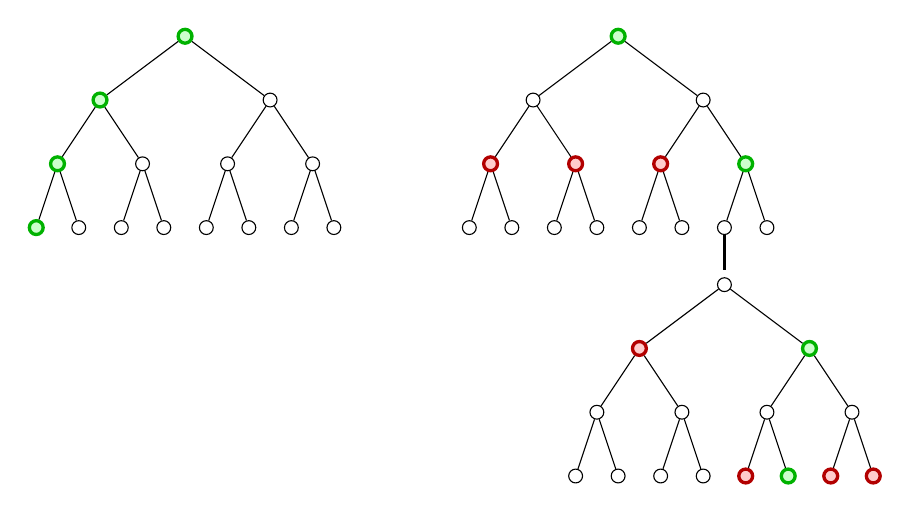
\begin{tikzpicture}[grow=down,level distance=0.9cm,
        base/.style={circle,draw,minimum size=5pt,inner sep=1.2pt},
        marked/.style={base,draw=green!70!black,fill=green!20,very thick},
        failed/.style={base,draw=red!70!black,fill=red!20,very thick},
        every node/.style=base,
        level 1/.style={sibling distance=2.4cm},
        level 2/.style={sibling distance=1.2cm},
        level 3/.style={sibling distance=0.6cm}]
        % First tree on the left
        \begin{scope}[xshift=-3cm,scale=0.9]
            \node[marked] (a0) {}
                child { node[marked] (a1) {}
                    child { node[marked] (a2) {} child { node[marked] (a3) {} } child { node {} } }
                    child { node {} child { node {} } child { node {} } }
                }
                child { node {} child { node {} child { node {} } child { node {} } } child { node {} child { node {} } child { node {} } } };
        \end{scope}

        % Second tree in the middle; its marked leaf becomes the root of the third tree
        \begin{scope}[xshift=2.5cm,scale=0.9]
            \node[marked] (b0) {}
                child { node {} 
                    child { node[failed] {} child { node {} } child { node {} } } 
                    child { node[failed] {} child { node {} } child { node {} } } }
                child { node (b1) {}
                    child { node[failed] {} child { node (b3) {} } child { node (b4) {} } }
                    child { node[marked] (b2) {}
                        child { node (b5) {}}
                        child { node (b6) {} }
                    }
                };

            % Third tree hanging from the marked leaf b3
            \begin{scope}[shift={(b5.south)},yshift=-0.7cm]
                \node (c0) {}
                    child { node[failed] (c1) {}
                        child { node (c2) {} child { node {} } child { node {} } }
                        child { node {} child { node {} } child { node {} } }
                    }
                    child { node[marked] {} 
                        child { node {} child { node[failed] {} } child { node[marked] {} } } 
                        child { node {} child { node[failed] {} } child { node[failed] {} } } 
                    };
                \draw[very thick] (0,0.7cm) -- (0,0.2cm); % small connector back to b3
            \end{scope}
        \end{scope}
    \end{tikzpicture}
    }
    \visible<3>{
    \begin{itemize}
        \item Note: there is new cost at finding the first match from the critical prefixes.
    \end{itemize}
    }
\end{frame}
